\documentclass[a4paper,12pt,final]{hitec}
\usepackage[english]{babel}
\usepackage{etex}
\usepackage{times}
\usepackage{setspace}
\usepackage{inputenc}
\usepackage{amssymb}
\usepackage{amsfonts}
\usepackage{amsmath}
\usepackage{graphicx}%[pdftex]
\usepackage{wrapfig}
\usepackage{subfig}
\usepackage{alltt}
\usepackage{moreverb}
%for more info on hyperref package see http://en.wikibooks.org/wiki/LaTeX/Packages/Hyperref
%\usepackage[pdftex,colorlinks=true,linkcolor=blue]{hyperref}
\usepackage{eso-pic}
% tikz related packages to provide scalable graphics 
\usepackage{tikz}
\usetikzlibrary{calc,mindmap,backgrounds,positioning,arrows,shapes,shapes.arrows,shapes.misc,automata,petri,patterns,scopes,chains,matrix,decorations.pathmorphing,shadows,calc}

%%%%%%%%%%%%%%%%%%%%%%%%%%%%%%%%%%%%%%%%%%%%%%%%%%%%%%%%%%%%%%%%%%%%%%%%%
%%%%%%%%%%%%%%%%%%%%% progrma code formattin environment %%%%%%%%%%%%%%%%
%%%%%%%%%%%%%%%%%%%%%%%%%%%%%%%%%%%%%%%%%%%%%%%%%%%%%%%%%%%%%%%%%%%%%%%%%
\usepackage{listings}
\usepackage{float}
\usepackage{caption}
%allows use of "@" before \begin{document}
\makeatletter
% this creates a custom and simpler ruled box style
\newcommand{\floatc@simplerule}[2]{{\@fs@cfont #1 #2}\par}
\newcommand\fs@simplerule{\def\@fs@cfont{\bfseries}\let\@fs@capt\floatc@simplerule
  \def\@fs@pre{}%\hrule height.4pt depth0pt \kern4pt
  \def\@fs@post{}% \kern4pt\hrule height.4pt depth0pt \kern4pt \relax
  \def\@fs@mid{}% \kern4pt
  \let\@fs@iftopcapt\iftrue}

% this code block defines the new and custom floatbox float environment
\floatstyle{simplerule}
\newfloat{program}{thp}{lop}
\floatname{program}{Listing}
\definecolor{codebgcolor}{HTML}{FFF3BC}
\definecolor{dkgreen}{rgb}{0,0.3,0}
\definecolor{gray}{rgb}{0.5,0.5,0.5}
\definecolor{mauve}{rgb}{0.58,0,0.82}
\newenvironment{code}[2]
{\begin{program}
  \vspace*{5pt}
  \captionsetup{format=plain,justification=centering,labelsep=colon,labelfont=bf,singlelinecheck=false,indention=0pt,position=below}
  \caption{#1}\label{#2}  
  \begin{center}
    \begin{tikzpicture}
      \node [fill=dkgreen!10!white,rounded corners=5pt]
      \bgroup
      \bgroup
      \begin{tabular}{l}}
      {\end{tabular}
      \egroup
      \egroup;
    \end{tikzpicture}
  \end{center}
\end{program}
}
%%%%%%%%%%%%%%%%%%%%%%%%%%%%%%%%%%%%%%%%%%%%%%%%%%%%%%%%%%%%%%%%%%%%%%%%%

%%%%%%%%%%%%%%%%%%%%%%%%%%%%%%%%%%%%%%%%%%%%%%
%%%%%%%%%%% Backgound picture %%%%%%%%%%%%%%%%
%%%%%%%%%%%%%%%%%%%%%%%%%%%%%%%%%%%%%%%%%%%%%%
\newcommand\BackgroundPic{
\put(-15,0){
\parbox[b][\paperheight]{\paperwidth}{%
\vfill
\centering
  %\includegraphics[width=1.1\paperwidth,height=1.1\paperheight, keepaspectratio]{sections/00-toc/images/background-new}%
\vfill
}}}

\newcommand\EveryPageBackgroundPic{
\put(-2,17){
\parbox[b][\paperheight]{\paperwidth}{%
\vfill
\centering
  %\includegraphics[width=1.0\paperwidth,height=1.0\paperheight, keepaspectratio]{sections/00-toc/images/every-page}%
\vfill
}}}
%%%%%%%%%%%%%%%%%%%%%%%%%%%%%%%%%%%%%%%%%%%%%%

\begin{document}  
  \setstretch{1.2}
  \begin{titlepage}
\title{Trident Genesis Platform Architecture from Engineering Perspective}
\company{Fielden Management Services Pty. Ltd.}
\author{TG Team}
\date{Lviv-Melbourne, 2011}
\maketitle
\clearpage
  This article provides a high level overview of the motivation, principle approaches and core features of the Trident Genesis software platform.
  The main emphasis is made on architectural and technological innovations, which together define a unique technology for the development and reliability improvement of business oriented applications.

\clearpage
\tableofcontents
\clearpage

\end{titlepage} % this file contains the title page and the abstract  
  \AddToShipoutPicture{\EveryPageBackgroundPic}
  \setcounter{page}{4} % need to reset page counter as by default after toc it start with 1 again 
  % using \input insterad of \include in order not statr every section from new page
  % need to include an image of the business rules to mind to code transition
\section{Motivation -- the ``why'' behind Trident Genesis}\label{sec:01}
  Software information systems\footnote{
    In this article the terms \emph{information system} and \emph{software application} are used interchangeably.
  } 
  (IS) are ubiquitous in modern society, which makes the ability to create and maintain reliable software critical from both consumer and manufacturer perspectives.
  The ideas and facilities built into a software application fully determine its purpose and value to the consumer (end user).
  That's why the subject of this article is the technological innovations, which are combined to provide a unique technology for the development of reliable business oriented information systems -- the Trident Genesis Platform (TG).

  \begin{wrapfigure}{r}{80mm}
    \centering    
    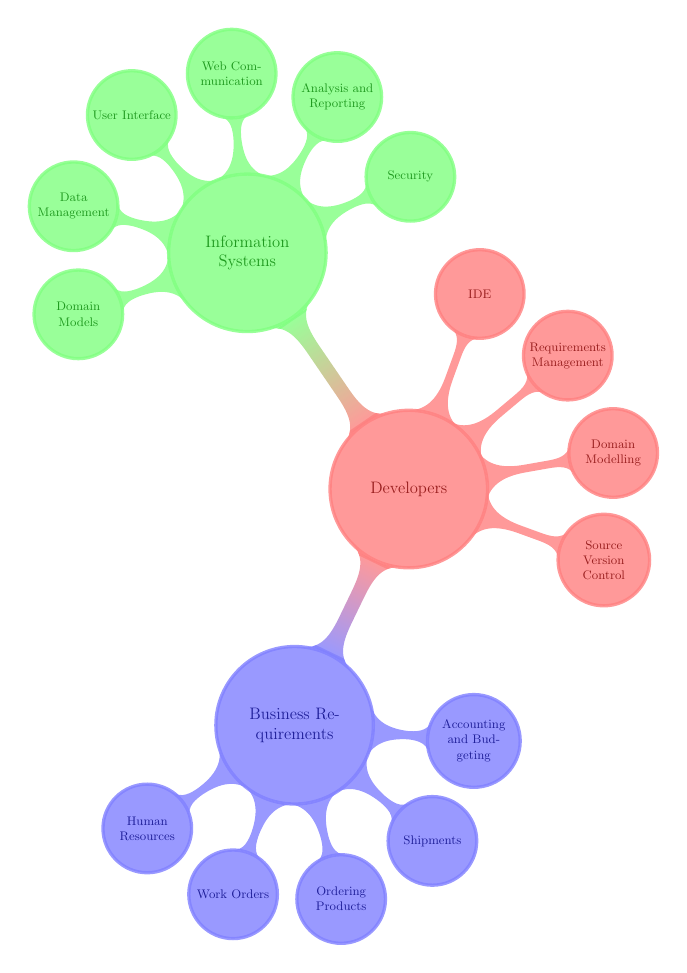
\begin{tikzpicture}[mindmap, opacity=0.8, scale=0.5, outer sep=0pt, transform shape]

      \begin{scope}[mindmap, concept color=green!50!white, text=green!50!black, level 1 concept/.append style={level distance=130, sibling angle=35}]
	\node [concept] at (-1.0, 2.0) (is) {Information Systems}[clockwise from=200] 
	  child {node [concept] (log) {Domain Models}}
	  child {node [concept] (alg) {Data Management}}
	  child {node [concept] (log) {User Interface}}
	  child {node [concept] (img) {Web Communication}}
	  child {node [concept] (opt) {Analysis and Reporting}}
	  child {node [concept] (res) {Security}};
      \end{scope}

      %\node (dev) at (2.1,-4) [circle, minimum size=4cm,fill,draw,thick,color=red!50, text=red!50!black] {Developers};
      \begin{scope}[mindmap, concept color=red!50, text=red!50!black, level 1 concept/.append style={level distance=150, sibling angle=30}]
	\node [concept] at (3.1,-4) (dev) {Developers}[clockwise from=70] 
	  child {node [concept] (ide) {IDE}}
	  child {node [concept] (req) {Requirements Management}}
	  child {node [concept] (dom) {Domain Modelling}}      
	  child {node [concept] (src) {Source Version Control}};
      \end{scope}

      \begin{scope}[mindmap, concept color=blue!50, text=blue!50!black, level 1 concept/.append style={level distance=130, sibling angle=35}]
	\node [concept] at (0.2,-10.0) (bus) {Business Requirements}[clockwise from=-5] 
	  child {node [concept] (accbud) {Accounting and Budgeting}}
	  child {node [concept] (ship) {Shipments}}
	  child {node [concept] (ord) {Ordering Products}}
	  child {node [concept] (work) {Work Orders}}      
	  child {node [concept] (hum) {Human Resources}};
      \end{scope}
    % 
    % Connections 
      \path (bus) to[circle connection bar switch color=from (blue!50) to (red!50)] (dev);
      \path (dev) to[circle connection bar switch color=from (red!50) to (green!50)] (is);
    \end{tikzpicture}
  \end{wrapfigure}

  First of all, it is important to understand what motivated the creation of TG and thus determined its main purpose.
  The evolution of computers led to an increase in computational power, which facilitated a significant increase in the amount of data that can be processed, and at the same time led to a need for a higher level of abstractions when creating software applications.
  Programming languages are at the core of software development, which also evolved -- from machine and assembly languages to modern mainstream programming languages such as Java, Scala, C\#.
  However, due to their nature all programming languages are convenient for instructing the computers how to perform specific computations, but not convenient for describing (modelling) the actual problem domain of the business being automated\footnote{Business for which an information system is being created.}.
  
  This leads to a huge semantic gap between the business requirements (what needs to be solved) and the actual solution (information system), which constitutes itself as a set of instructions to the computer.
  The two sides of the gap are bridged only by the software developers who have built the solution and hold the transition model in their minds.
  So the software developers serve as translators between the language of the business domain and the language of the software information system.
  Due to this and the fact that the same business requirements can be expressed in multiple ways using a general purpose programming language, there are many problems maintaining the solution, especially when the original developers are not around.

  In his paper ``Language Oriented Programming'', M.~P.~Ward points to several important research results:
  \begin{itemize}
    \item There is a thin spread of domain knowledge among software developers in most projects;    
    \item Most development is maintenance. 
	  System evolution is so common, that development from scratch is the exception rather than the rule;
    \item Most specifications are incremental. 
	  The customer is rarely able to provide a complete specification at any stage of the project;
    \item Domain knowledge is important;
    \item There is a gulf between developer and user. 
	  Few developers have adequate knowledge about the user's work. 
	  This leads to major misconceptions about the system's purpose.
  \end{itemize}
  
  To date most of the development of business applications involves low-level technical details, which deprive developers of the time to think and work on the actual business requirements.
  
  The above problems and our own experiences of having to deal with them on a daily basis led to the need of raising the level of abstraction that would hide low-level technical details and provide a uniform programming model for implementing software solutions as close as possible to the business terminology.
  By raising the level of abstraction the TG platform brings closer together software developers and business domain specialists, which is one of the platform's less obvious but defining features.
 %
  \section{Platform \& Business Applications}\label{sec:02}  

  The notion of the ``platform'' and ``platform-oriented'' software development is nowadays well accepted and in most cases is understood more generically than a capability to operate in a specific operating system.
  Usually, ``platform'' is understood as an execution environment and a set of technologies used for developing software applications for a certain domain.
  Any software application can be based on several platforms, which can be visualised as layers placed on top of each other with an actual application at the very top.
  What is defining for any platform is its unique model that isolates software developers from the details of lower level technologies and platforms.

  \begin{wrapfigure}{r}{55mm}
    \centering    
    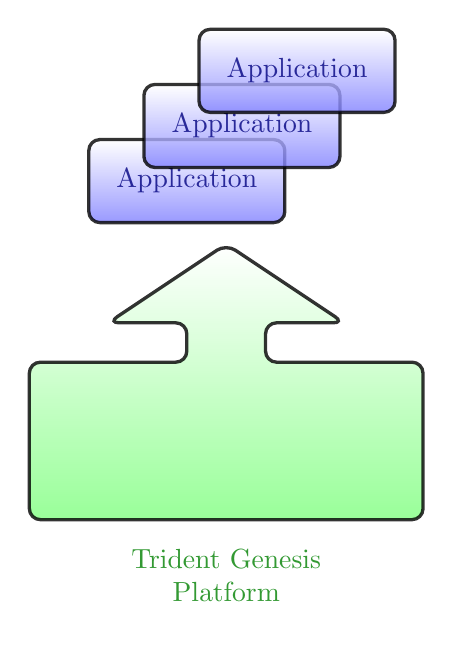
\begin{tikzpicture}[node distance=1cm, auto, opacity=0.8]
      \tikzset{
	  mynode/.style={rectangle,rounded corners,draw=black, top color=white, bottom color=blue!50,very thick, inner sep=1em, minimum size=3em, text centered, text=blue!50!black},
	  platform/.style={rectangle,rounded corners,draw=black, top color=white, bottom color=green!50!white,very thick, inner sep=1em, minimum size=3em, text centered, text=green!50!black}
      }  
      \node at (1, 1) [mynode] (ap1) {Application};
      \node at (1.7, 1.7) [mynode] (ap1) {Application};
      \node at (2.4, 2.4) [mynode] (ap1) {Application};

      \def\platformpath{-- +(5cm,0cm) -- +(5cm,2cm) -- +(3cm,2cm) -- +(3cm,2.5cm) -- +(4cm,2.5cm) -- +(2.5cm,3.5cm) -- +(1cm,2.5cm) -- +(2cm,2.5cm) -- +(2cm,2cm) -- +(0cm,2cm) -- cycle}
      \draw (-1,-3.3) [platform] \platformpath 
	    node [below,text width=7em, text centered,xshift=2.5cm] {Trident Genesis Platform};  
    \end{tikzpicture} 
  \end{wrapfigure}
  
  From this perspective Trident Genesis is not different providing a necessary abstraction for using lower level technologies without changing the source code of a business application.
  For example, it provides the developers with its own model for working with data, which abstracts out the specifics of a particular database.
  This facilitates using different databases without modifying the business application source code.
  A small-scale application can happily use H2 or MySQL, while a large-scale application would work with Oracle Database or MS SQL Server.

  At the very beginning the TG platform was targeted at inhouse purposes for migrating existing and developing new business applications.
  Such practical-driven approach allowed capturing the existing experience building business application in a way that made TG not just a set of reusable components and libraries, but a complete application platform covering every aspect of the application development and deployment life-cycle.
  This in turn positioned TG as a standalone product, which does not mix in any specifics of a particular business application and provides a generic way for building diverse business-oriented information systems.

  The TG platform incorporates well thought out set of features sufficient for providing solutions to a large variety of business tasks/problems.
  This results in reliable and controlled interoperability between underlying technologies governed by the platform without the need for introducing external dependencies resulting in ``stitches'', which often become the cause of many software defects.
  An excellent example of such interoperability is the developed \emph{type system}.
  When building applications on top of TG, developers use the provided system of types for interacting with web-resources, databases and for implementing business logic as well as the user interface.
  This removes the need for developers to work on type transformations when implementing different layers of the information system.
  
  As has been outlined earlier, the majority of software applications are not created from scratch, but enhanced and modified as business demands.
  Especially for business applications it is critical to support their efficient customisation by developers not involved in the original construction of the system.
  This situation defines a special requirement for such systems to be easily comprehended, which has been taken into account when designing the TG platform.
  Building applications on top of TG provides a clear separation between technical and business aspects of software applications catering for their much higher level of customisability in order to meet customers' requirements. %
  \section{Types and Metadata == Business Modeling}\label{sec:02}

  In recent years there was a spike in popularity of the Domain-Specific Languages (DSL) concept, which can be explainded by the programming issues outlined in the introduction, which affect not only the business oriented information systems, but also other domains dependent on various informations systems.

  The concept of DSL is not new.
  In fact, there are well established solutions for business software what exist for a long time and explictly utilise this concept.
  For example, SAP Business Suite offers a specialised language ABAP and Microsoft Dynamics Axapta provides X++.
  These are examples of so called \emph{external DSL}, which are separate or external to the programming language used natively for creation of the mentioned products.
  The main disadvantage with external DSLs is this: if there is a need to express a complex algorithm the expressive power of a DSL should be adequate to implement such algorithm, which in turn makes that DSL yet another general purpose programming language.
  
  An opposite to external DSL is the concept of \emph{interna DSL} -- a specialised language, which utilises the capabilities of a specific general purpose programming language of expressing language-like constructs that can be used together with the general purpose programming language.
  Internal DSLs share the development and execution infrastructure of the corresponding general purpose programming language taking a significant advantage of reusing debugging, profiling tools, code editors, existing programming libraries etc.
  
  Different general purpose programming languages provide different degrees of support for developing sophisticated internal DSLs.
  For example, scripting languages generally provide better ways of implementing internal DSLs (e.g. Ruby).
  However, in our strong oppinion statically type langugages are of essential importantce for constructing complex business oriented information systems.
  
  From the very beginning the Trident Genesis Platform was envisaged as an application platform founded on the concept of internal DSLs and domain-driven development.
  It was decided to tap into the power of modern IDEs and existing programming skills of software developers, which resulted in the choice of Java as the host general purpose programming language\footnote{Java does not provide the best support for developing internal DSLs (e.g. Scala is a lot more adequate), but the maturity of the existing Java infrastructure and development experience played a critical part in this decision.}.

%   \begin{figure}[!htp]
%     \centering
%     
\includegraphics[width=10cm]{sections/01-intro/images/00-splash.jpg}
%     \caption{Example of an Embedded Image}\label{fig:01}
%   \end{figure}


%  // calculates the average yearly maintenance cost (for the last 3 years) per sectors of NORTH division. Only vehicles of MERCEDES make and models starting from 315 or 316 or VITO model are taken into account.
%         select(WorkOrder.class).
%         where(). //
%         prop("vehicle.model.make.key").eq().val("MERCEDES").and().
%         begin().prop("vehicle.model.key").starts_with().any_of_values("315", "316" ).or().prop("vehicle.model.key").eq().val("VITO").end().and().
%         year_of().prop("actualStart").in().values(2009, 2010, 2011).and().
%         prop("vehicle.station.zone.sector.division.key").eq().val("NORTH").
%         yield_and_group().prop("vehicle.station.zone.sector").as("sector").
%         yield().begin_expr().sum_of().prop("actualCost").div().val(3).end_expr().as("averageYearlyMaintenanceCostPerSector").model_as_aggregate();
  %
  \section{Data Management \& Web Resources}\label{sec:04}

  One of the central differentiators of business applications from other information systems is their paradigm for data processing.
  Data related activities is the most important and at the same time the most vulnerable part of business applications.
  Vulnerability can be explained by the lack of~~``close to perfection'' solutions unlike for some other types of software systems such as word processing or digital painting software.
  Business applications are constantly under the pressure of contradicting requirements.
  On the one hand, there is a need for processing large datasets, while on the other hand business applications should demonstrate good performance and rich functionality.
  The amount of data to be processed always increases, requirements for more diverse functionality occur constantly and the need for high scalability of business applications is ever increasing.
  
  There are several well accepted data processing paradigms currently in use for developing business applications.
  However, there is no single best solution that would satisfy all business requirements.
  It can be observed that most if not all available solutions implement different combinations of data management paradigms, which represent compromises to improve certain specifically targeted characteristics.

  With the increase of the role of the Internet as a communication mechanism for Enterprises as well as the maturity of many Internet technologies, business applications are required to process data not only by directly communicating with databases\footnote{Usually RDBMS.}, but also distributed across the Web resources.
  This introduced an additional layer of complexity where in most cases developers need to switch between paradigms of working with relational databases and Web resources.

  The Trident Genesis platform introduces its own data processing solution by reusing some of existing paradigms in its own unique way to provide a uniform programming model for data processing against both databases and web resources\footnote{Web resources developed using the Trident Genesis platform.}.
  All data CRUD (create, request\footnote{Commonly, ``R'' stands for \emph{read} or \emph{retrieve}, but here we'd like to emphasise a more rich functionality behind the ``R'' in TG as described farther in the text.}, update, delete) operations utilise pure object-oriented approach combined with carefully designed internal DSL called ``Entity Query Language''.
  This means that developers do not operate on database records or web resources directly.
  Instead they are confined to the much higher conceptual level of business domain models and the query language that operates directly on these models.
  
  For example, in order to modify persisted data there is no need to write complex low level queries and translate their result into the business domain model.
  Persisted business entities are requested declaratively, modified by changing their properties at the object level and saved also declaratively.
  The platform fully takes care of handling low technical details for translating declaratively expressed actions into corresponding Web or database related API calls.
  Such development model provides a convenient way to implement business rules related to changes of domain entities such as validation, before and after save logic, which can lead to modification of additional entities if required etc.
  It also fully supports both \emph{remote} and \emph{local}\footnote{The \emph{remote} here means the server-side application, and \emph{local} -- the client-side application running on users' local machines.} data processing, which provides developers with a flexible way to leverage computational resources by controlling how ``thin'' should their business client and server applications be.

  \subsection{Client- \& Server-Side Applications}
  With an advent of multi-tier software architecture, the three-tier architecture became a de-facto standard for developing web-enabled applications.
  The current state and trend in Web development technologies is twofold: on one side there is an ``in-browser HTML'' model, where client applications are served as a web page, on another -- rich client application model, where client applications are fully capable desktop applications.
  Both models have their strengths and weaknesses.

  As mentioned above, the enforced by the platform programming model strives for uniformity. 
  The platform follows the path of reducing the number of concepts and technologies needed for development of business applications.
  One of the key aspects of this, is the use of Java as the only programming language required to develop business applications with TG.
  This is achieved by utilising the RIA paradigm for developing both client and server applications using only the Java programming language.
  
  From a practical perspective of software development this has a significant advantage over the ``in-browser HTML'' model.  
  For example, such important activities as debugging and profiling are performed in a familiar environment of the preferred IDE, where developers think in terms of their primary programming language instead of handling the complexity of context switching between several languages\footnote{E.g. Java for the server application and Java Script for the client application.}.
  At the same time, the end-users of business applications benefit from the power of the fully fledged JVM utilised by the client-side application to provide high performance and excellent usability experience.
  
  The server-side represents a set of loosely coupled Web resources that adhere to principles of the Resource Oriented Architecture.
  This architectural style lends itself very well to develop scalable business applications, which can leverage different deployment infrastructures -- from a single server machine to a cluster of multiple machines and the cloud.
  The provided development model hides the technical complexity of developing Web resources\footnote{Platform supports the development of custom Web resources if required, but such need is unlikely due to rich semantics of the provided domain level abstractions.} by treating all domain entities as such.
  The platform understands the application execution context automatically choosing the appropriate handling mechanism of domain entities either as ordinary Java objects in the local memory or as Web resources residing at the server side.
  
  For example, if the business application attempts to save a domain entity\footnote{It could either be persistent or synthetic entity, which is possible due to the platform's uniform development model.}, the underlying platform mechanism would determine the origin of the request, resulting in either a call to the database for the server-side application or a corresponding Web resource for the client-side application.
  All of this is accompanied by automatic transaction demarcation ensuring referential integrity of the data.

   \begin{figure}[!h]
    \centering    
    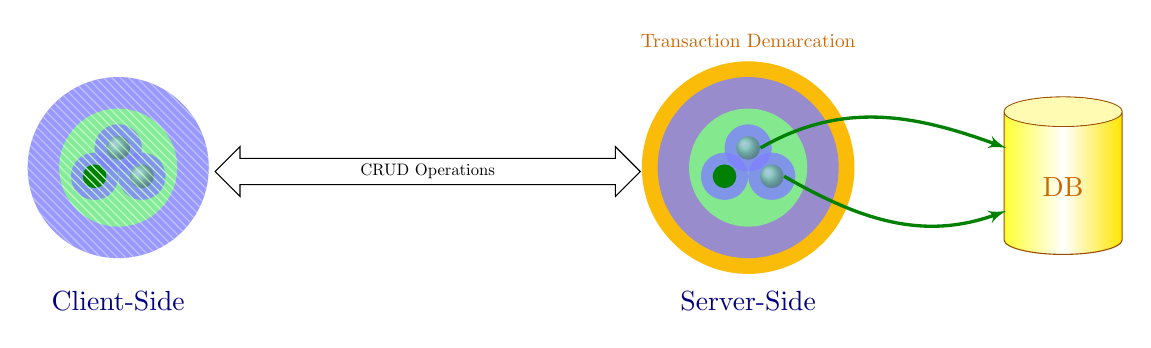
\begin{tikzpicture}[>=latex']
      \tikzset{
	  outercore/.style={circle, fill=blue!50!white, inner sep=0em, minimum size=0.6cm},
	  core/.style={circle, shade, ball color=green!50!white, inner sep=0em, minimum size=0.3cm},
	  score/.style={circle, fill=green!50!black, inner sep=0em, minimum size=0.3cm},
	  outer/.style={circle, fill=blue!50!white, inner sep=0em, minimum size=2.3cm},
	  inner/.style={circle, fill=green!50!white, inner sep=0em, minimum size=1.5cm},
	  trans/.style={circle, fill=yellow!50!orange, inner sep=0em, minimum size=2.7cm}
      }

      %-----#1 height, #2 width, #3 aspect, #4 name of the node, #5
      %-----coordinate, #6 label
      \def\aboxl[#1,#2,#3,#4,#5]#6{%
	\node[draw, cylinder, alias=cyl, shape border rotate=90, aspect=#3, %
	minimum height=#1, minimum width=#2, outer sep=-0.5\pgflinewidth, %
	color=orange!60!black, left color=yellow!80, right color=yellow!80!orange, middle
	color=white] (#4) at #5 {};%
	\node at #5 [orange!80!black] {#6};%
	\fill [yellow!30] let \p1 = ($(cyl.before top)!0.5!(cyl.after top)$), \p2 =
	(cyl.top), \p3 = (cyl.before top), \n1={veclen(\x3-\x1,\y3-\y1)},
	\n2={veclen(\x2-\x1,\y2-\y1)} in (\p1) ellipse (\n1 and \n2); }
      
      \begin{scope}[pattern=dots]
	\node (o) at (0, -0.25) [outer, opacity=0.8][postaction={pattern=north west lines,pattern color=blue!20}] {};      	
	\node (i) at (0, -0.25) [inner, opacity=0.8,][postaction={pattern=north west lines,pattern color=green!20}] {} node [below,text=blue!50!black,yshift=-1.7cm] {Client-Side};

	\begin{scope}[scale=0.3]
	  \node (t) at (0,0) [outercore, opacity=0.8][postaction={pattern=north west lines,pattern color=green!20}] {};	
	  \node at (0,0) [core, opacity=0.5][postaction={pattern=north west lines,pattern color=green!20}] {};

	  \node (r) at (1,-1.2) [outercore, opacity=0.8][postaction={pattern=north west lines,pattern color=green!20}] {};	
	  \node at (1,-1.2) [core, opacity=0.5][postaction={pattern=north west lines,pattern color=green!20}] {};

	  \node (l) at (-1,-1.2) [outercore, opacity=0.8][postaction={pattern=north west lines,pattern color=green!20}] {};	
	  \node at (-1,-1.2) [score][postaction={pattern=north west lines,pattern color=green!20}] {};
	\end{scope}
      \end{scope}

      \begin{scope}[xshift=8cm]       
	\node[trans] at (0, -0.25) {} node [above,text=orange!80!black, scale=0.7,yshift=1.7cm] {Transaction Demarcation};;
	\node (o2) at (0, -0.25) [outer, opacity=0.8] {};
	\node (i2) at (0, -0.25) [inner, opacity=0.8] {} node [below,text=blue!50!black,yshift=-1.7cm] {Server-Side};

	\begin{scope}[scale=0.3]
	  \node (t2) at (0,0) [outercore, opacity=0.8] {};	
	  \node (t2c) at (0,0) [core, opacity=0.5] {};

	  \node (r2) at (1,-1.2) [outercore, opacity=0.8] {};	
	  \node (r2c) at (1,-1.2) [core, opacity=0.5] {};

	  \node (l2) at (-1,-1.2) [outercore, opacity=0.8] {};	
	  \node at (-1,-1.2) [score] {};
	\end{scope}	
      \end{scope}     
      \begin{scope}[xshift=3.93cm,yshift=-0.3cm]
	\node[shape=double arrow,draw,minimum height=9cm,scale=0.6] {CRUD Operations};
      \end{scope}
      \begin{scope}[xshift=12cm,yshift=-0.5cm]
	\aboxl[2.0cm,1.5cm,1.6,a1,(0,0)] {DB};
	\node [xshift=-0.6cm, yshift=0.5cm] (mark1) {};
	\node [xshift=-0.6cm, yshift=-0.3cm] (mark2) {};
      \end{scope}


      \fill [very thick, green!50!black,->,out=30,in=160] (t2c.east) edge (mark1.west);      
      \fill [very thick, green!50!black,->,out=-30,in=-160] (r2c.east) edge (mark2.west);
    \end{tikzpicture}   
  \end{figure}


  \subsection{Entity Query Language}
  
  The platform ensures an effective technological support of the object-oriented programming approach, which underpins the provided development model.
  One of the principal solutions incorporated into the platform is \emph{Entity Query Language} -- a declarative query language based on SQL that provides a number of significant enhancements. 
  The primary objective of these enhancements is the support for working with business entities in a natural for object-oriented programming way, which ensures effective and ergonomic means for implementing business solutions.
  
  One of the key benefits of the object-relational paradigm for data management is its clarity and simplicity for developing applications.
  Object-orientation provides excellent readability of algorithms implementing the business logic, significantly reduces the number of programming errors and ensures data integrity at a high level.
  
  Entity Query Language (EQL) represents an internal Java DSL, which embraces the fluent interface concept and object composition to provide a type safe query language that matches the data processing power of SQL, but exceeds it in clarity and expressiveness.
  This provides a natural way to express data processing instructions in terms of the business domain instead of the low level data structures.
  The implementation of EQL as an internal DSL automatically takes advantage of modern Java IDEs, which provide code highlighting, code insight etc.
  This favourably differentiates EQL from alternatives such as Hibernate Query Language where queries are expressed as strings without any semantics for an IDE or compiler to validate them at design time.
  Thus, every EQL query is validated at design/compile time naturally fitting into the Java's statically typed nature.
  
  An example of an EQL query is provided as code listing~\ref{lst:eql}.  
  It calculates the average yearly (over the period from 2009 to 2011) maintenance cost of vehicles manufactured by ``MERCEDES'' and their model names starting with ``315'', ``316'' or ``VITO'', for every sector of division ``NORTH''\footnote{This example is specific to a certain fleet domain and the full comprehension of the query implies good understanding of that domain.}.  

  \lstset{language=Java,morekeywords={val,select,where,prop,eq,and,begin,end,starts_with,any_of_values,values,or,yield_and_group,as,yield,begin_expr,sum_of,div,end_expr,model_as_aggregate,year_of,in},numbers=left, numberstyle=\tiny, basicstyle=\scriptsize, stepnumber=1, numbersep=5pt, keywordstyle=\color{dkgreen}, stringstyle=\color{blue}}
  \begin{code}{EQL Query Example}{lst:eql}
  \begin{lstlisting}
    select(WorkOrder.class).
    where().
    prop("vehicle.model.make.key").eq().val("MERCEDES").and().
    begin().
      prop("vehicle.model.key").starts_with().any_of_values("315", "316").or().
      prop("vehicle.model.key").eq().val("VITO").
    end().and().
    year_of().prop("actualStart").in().values(2009, 2010, 2011).and().
    prop("vehicle.station.zone.sector.division.key").eq().val("NORTH").
    yield_and_group().prop("vehicle.station.zone.sector").as("sector").
    yield().
      begin_expr().
	sum_of().prop("actualCost").div().val(3).
      end_expr().as("averageYearlyMaintenanceCostPerSector").
    model_as_aggregate();
  \end{lstlisting}
  \end{code}
  
  The demonstrated EQL query is interesting in many ways.
  It shows proper support for working at the domain level referencing the nested structure of domain entities, multiple EQL constructs (aggregation, grouping, logical operations) and the capability of working with expressions\footnote{
    Expressions in TG are implemented as an internal DSL for the use by developers as well as external DSL for the use directly from business applications by power users. 
    All arithmetical operations, specially provided functions (e.g. year\_of(date)) and aggregations can be represented as type safe expressions.
  }
  (summation of property actualCost divided by 3).  
  
  Less obvious, but very powerful feature demonstrated in this query, is the ability to produce dynamically composed results that do not necessarily match any of the pre-built domain entity types.
  This capability is critical for many real-life business requirements where some business logic or analysis may require ad-hoc data retrieval without modifying the domain itself.
  The declarative nature of EQL significantly simplifies creation of complex queries with nested sub-queries, grouping and aggregation, which is extremely important for implementing analytical solutions.  

  Entity Query Language fully reuses the metadata associated with domain entity types.
  This facilitates dynamic optimisation of query execution at the databases level, which is possible due to semantic transition between metadata of the domain and SQL.
  For example, if some property of a domain entity, which represents a reference to other domain entity, is declared as required, then the query execution mechanism would recognise such reference as SQL's \emph{INNER JOIN} instead of \emph{OUTER JOIN}, which significantly speeds up query execution.

  The EQL execution mechanism works equally well with small and large datasets by supporting partitioned data loading.
  This does not require any additional work on part of developers -- they just need to provide the query and the system would automatically execute it with the necessary level of granularity.
  It is important that the platform does not rely on any RDBMS vendor specific features such as cursors, which might require keeping resulting datasets open in memory.
  Instead, the EQL execution mechanism automatically enhances queries to retrieve data sequentially.
  This approach naturally fits into the stateless Resources Oriented Architecture of the platform to properly support scalability of TG-based applications.

  Developers working directly with SQL always ensure that only the required data should be returned as the result of query execution.  
  Trident Genesis supports fine-tuning of EQL queries that match flexibility of SQL.
  Unlike, many other existing object-relational technologies that either follow the lazy-loading model\footnote{
  This causes severe performance issues known as ``$n+1$ request'', which is especially dangerous when the technology is used by novice developers.}
  or provide ways to specify fetching as part of queries\footnote{Or even more restrictively -- as part of the object-relational mapping.}, the platform supports a concept of the \emph{explicit fetching strategy}.
  This separates EQL queries, which indicate how to find data, from the fetching models, which indicate what data exactly needs to be returned providing a full control over the resulting object graph initialisation.
  So, depending on business requirements the same EQL query can be executed with different fetch models, which provides a way to optimise the load time and memory footprint.

  As mentioned before, the development model hides many technical details including the data communication mechanism.
  This completely removes the conceptual mismatch between the ways of querying the domain against databases and Web resources.
  Any EQL query can be seamlessly executed as part of either client- or server-side applications.
  Thus, EQL provides a uniform high-level domain oriented communication concept. %
  \section{Domain-Driven UI Model}\label{sec:05}

  User interface (UI) serves an important role for business applications.
  There are two reason for this:
  \begin{itemize}
   \item For a large number of enterprise employees, a business application represents the main application used during the day. 
	 These people work with the business application for a good portion of their working day, but at the same time they aren't necessarily the savvy computer users.
   \item Usually, UI of business applications constitutes a large part of the final solution having multiple forms, tabsheets, menus etc.
  \end{itemize}
  Unlike other types of software systems, business applications contain hundreds of forms, which may change over time as the result of application evolution and changes to business rules.
  This results in a considerable effort to develop and support UI of business applications.
  Acknowledging the above, Trident Genesis incorporates a full support for domain-driven UI development into the provided programming model.
  It provides a number of mechanisms for rapid development of uniform user interfaces, which includes windowing model, a system of forms, type-aware UI controls, user notification mechanism, implicit multi-threading model etc.
  
  The principle idea behind building UI in TG, is a full reuse of metadata, type information and business logic controllers in order to support a nearly automatic UI construction with little involvement of the developer.
  As with any other aspect of TG-based development, when building user interfaces the developers work at the domain level instead of the low-level of UI controls while being provided with flexible ways to customise the form layout.
  So, the same type system and metadata used to model domain entities is used throughout the application development process.
  
  For example, when constructing UI, the developer simply requests a set of UI controls for a given domain entity.
  The platform automatically determines what controls are suitable for the properties of the specified domain entity.
  The returned UI controls are fully initialised based on the metadata and bound to the specified entity instance.
  Thus, all changes done to that instance programmatically would be reflected in the UI controls and vice versa.
  This mechanism adheres the domain model to the letter including execution of the specified validation business rules etc.
  A savvy reader should already notice that TG follows the Model-View-Controller architectural pattern when it comes to UI construction, which reuses all the platform's essential building blocks.

  One of the obvious advantages of this approach is the uniformity of UI -- properties of different domain entities with the same type are always represented by the same UI controls.
  This greatly facilitates familiarisation of end-users with TG-based applications, which is especially noticeable in cases where several business applications are used in the same organisation.
  This way users do no need to learn new UI controls, paradigms or deal with unexpected behaviour over the period of application evolution.
  Another less obvious advantage of such transparent approach, where UI controls are fully bound together with domain entities and corresponding business controllers, is a natural predisposition to the test-driven development.
  The developers need only to ensure correctness of business domain models and controllers while the views would uniformly reuse them.

  The platform's type system provides a clear definition of all possible combinations of properties used for modeling business domains.
  As outlined earlier, the most complex type is a domain entity itself, which may contain properties of different predefined types such as Date, Money, String as well as other domain entities.
  The well-defined type system and rules for its customisation served as the foundation for implementing a set of UI paradigms and controls providing a way for the platform to automatically determine both the visual representation and behaviour of the application user interface.
    
  For example, a UI control provided for editing of a property that is of a domain entity type is fully equipped with quick and advanced search capabilities.
  Such control does not require any configuration to be coded by the developer -- everything is automatically determined from the type and metadata of the property.
  Similar happens for properties of other types.
  As another example consider a property of type Date.
  The platform recognises the type and automatically associates it with a specially design Date/Time Picker UI control.
  In all cases developers do not need to provide any additional information -- just to layout UI controls on the form.
  
  There are only two principle high-level UI concepts for organising application User Interface:
  \begin{itemize}
   \item Entity Master -- a view for a single domain entity used specifically for review of its details, editing and creation of new ones.
	 There can be entity masters of varying complexity, which fully depends on the complexity of the underlying domain entity.
    \item Entity Centre -- a view for representing sets of domain entities of the same type. 
	  It is used for review of practically unlimited number of domain entity instances without loading all of them into memory, which is possible by reusing the EQL functionality outline earlier.
	  This view supports sophisticated configuration and filtering capabilities, ordering, data export functionality and more.
  \end{itemize}
  
  The platform provides a mechanism that orchestrates seamless integration of masters and centres into a cohesive system, where views are linked together based on domain entity type information allowing natural navigation between the views.
  For example, the mechanism of Entity Masters implements a strategy for semantic identification by making a correspondence between view and domain entities.
  This way a previously opened for a specific entity Entity Master gets activated instead of creating a new instance.
  Effectively, the platform offers developers a ready-to-use strategy for organising application user interface, which covers practically all scenarios required by the business domain.

  The above highlights only some UI solutions provided as part of the platform and there are more UI related features that could not all be described in this document.
  Platform's modularity ensures that UI controls and related logic cannot be mixed into domain models and implementation of the business logic.
  The most important aspect of the provided UI development model is that it represents a high-level solution, which fully reuses the business domain model.
  Such standard UI construction mechanism ensures the uniform user interface across all TG-based business applications.
  This allows efficient reuse of user experience.
  Users who understand principles and approaches of one TG-based application would easily start working with any other. %
  \section{Analytical \& Reporting Capabilities}\label{sec:06}
  Every business application has two main functions directly experienced by users through the application user interface:
  \begin{itemize}
   \item Data entry -- the mechanism, by which new facts from the real world get populated into the system\footnote{There could also be some means of automatic batch data imports, but these do not require any direct interaction with application users.};
   \item Data analysis and reporting -- the mechanism to support business decision making.
  \end{itemize}
  Historically these two functions had two different groups of users~-- data operators and business analysts.
  Often the data analysis and reporting functionality was facilitated by a different application than the one used for data entry.
  Here is a brief retrospective analysis suggesting the cause of such separation.
  
  The 1990s have established the relational database model as the de-facto standard for managing data within enterprises.
  This model is usually associated with a two-tier application architecture also known as the Client/Server Architecture\footnote{The modern definition of the three-tier model is also associated with the notion of a Client/Server Architecture.}.
  This had the effect where the modelling of business domains at the software level was thought of in terms of relational algebra, which served as the theoretical foundation for relational databases.
  At about the same time, object-oriented paradigms and programming languages were gaining ground, ultimately leading to the creation of the multi-tier architecture with the majority of business related modelling moved out of the databases and into the middle tier, which is typically implemented in an object-oriented programming language.
  The relational databases started to be used more as an efficient storage mechanism than a modelling paradigm.
  The object-oriented and relational models have a naturally occurring impedance mismatch, which is being resolved in various ways, including the programming model provided as part of the TG platform.
  
  Despite the fact that the core of modern business applications (domain model and business logic) is usually implemented using an object-oriented programming language, all current reporting and analytical tools operate directly on the database where the data is stored while completely disregarding the domain model present in the application's middle tier.  
  The reason for this is well understood -- there is no easy way for external tools to tap into the application's middle tier.
  At the same time relational database management systems support a number of standards (e.g. database languages such as SQL, and connectivity tools like JDBC and ODBC) providing well-defined means to interact with databases produced by different vendors.
  However working strictly at the database level leads to a large number of disadvantages, including the need to work with the low-level technical details of the database structure that the object-relational mechanism works so hard to hide, and the ability to produce reports based on SQL queries that do not correspond to the underlying domain model (e.g. join database tables in a way that the domain model at the middle tier prohibits).
  It is also often the case that the business analyst who works with a third-party tool to produce reports and analyses does not belong to the business application development team who worked closely together with domain experts to devise the system in the first place.
  This requires additional investment to familiarise the analyst with the business domain as well as the underlying database structures.
  Mixing object-oriented and relational approaches to work with the system in such a way brings back the object-relational impedance mismatch, which would otherwise have been carefully handled by the underlying frameworks.
  This leads to situations where modifications of business applications invalidate reports and analyses that were produced using third-party tools.

  The reporting technology provided by TG is unique from many perspectives.
  First of all, the platform does not have any special notion of a ``report building'' facility.
  The developer is provided with a range of platform mechanisms such as a type system (especially synthetic types), the power of EQL, and the domain-driven UI model, which can be used in different combinations to implement highly configurable and complex reports.
  Due to this fact, reports naturally fit into the application user interface.
  Effectively users do not need to differentiate between the reporting mechanism and other parts of the general-purpose application user interface.
  We strongly believe that seamless integration of reporting and data entry functionality is required for modern business applications due to the criticality of analytical information to different groups of users~-- those making business decisions, and those entering data into the system\footnote{This is especially relevant for the modern fast changing world where cross-skilled personnel are of the utmost importance to the success of the business.}.
  This approach organically shifts the reporting functionality away from  the ``paper'' paradigm, and towards interactive ``online'' and ``real-time'' processing.
  
  One of the most interesting platform mechanisms to support interactivity is the ability for users to directly operate on domain entities from the UI.
  This provides easy-to-use ad-hoc reporting functionality with multiple features such as aggregation, filtering, ordering, grouping and even dynamic enhancement of existing domain entities with new calculated properties\footnote{This change has a local nature and is confined to that specific report configuration, not affecting other parts of the system.}, without any knowledge of programming or even of a query language.
  Report results can be represented in a tabular manner, and also as charts and pivot tables with drill-down capabilities.
  There can be multiple configurations of the same report, which can be saved and shared between application users.
  Power users can use the full potential of such a reporting facility to create really complex and sophisticated reports.

  The Trident Genesis platform emphasises its domain orientation by proliferating the underlying business model throughout the application architecture.
  Not only does it provide developers with object-oriented means to model and interact with the business domain, but it also makes the domain explicitly visible to the application end-users.
  This particular trait is known as \emph{semantic transparency} of the business domain, which is perceived equally by both software developers and the application end-users.
  Such a approach purposely raises the user's level of awareness of the implemented business model, thus facilitating communication between application developers, users and domain experts\footnote{Who may or may not be application users.}, ultimately resulting in increased value for the business. %
  \section{Other Essentials \ldots}\label{sec:07}

  The platform provides other essential functionality that cannot be described in details as part of this document.
  In this section, we would like only to highlight some of it.

  \paragraph{Application Security.}
  The platform incorporates both authentication and authorisation mechanisms that govern application security.
  The authentication mechanism is heavily influenced by Amazon S3 token-based security schema in combination with RSA encryption.
  It works automatically out of the box and may require developers only to plug-in the server-side user identification model.
  The default model implementation, provided as part of the platform, stores all user credentials in the back-end database.
  Alternative application specific implementations may work with LDAP server or any other organisation specific mechanism.
  
  Unlike authentication, the authorisation mechanism is used more explicitly during application development, which is required to support fine-grained access control.
  The platform provides a unique declarative authorisation mechanism that ergonomically fits into the development model using the object-oriented paradigm.
  A concept of \emph{security token} represents a security demarcation mechanism, which can be applied to the smallest execution artifacts such as accessors to domain entity properties or any other method in the domain model.
  As opposite to many other existing technologies where the authorisation mechanism is often associated with UI controls, the platform unifies the authorisation mechanism with the business domain model.
  This way, no matter where in the application logic (including UI and other client- or server-side modules) a certain business functionality is accessed it is always protected.
  
  Security tokens are type safe and may form hierarchies by reusing the object-oriented mechanism of inheritance.
  This provides a convenient way to logically group security tokens.
  Another important concept is the \emph{security demarcation scope}.
  It provides an automatic conflict resolution for nested scopes of the application logic demarcated by security tokens with different permissions.
 
  The concept of semantic transparency is also applied to the authorisation mechanism.
  Application developers and administrators, who control user permissions, perceive security tokens in exactly the same semantic context.
  For example, this facilitates cooperation of these stakeholders to devise the most appropriate structure and scope for security tokens.

  \paragraph{Users \& Roles.} 
  All application users are based on the provided by the platform user model.
  Each TG-based application maintains identity of the currently logged in user, which covers both client- and server-sides\footnote{
    In order to support stateless server-side implementation, the platform does not maintain any user sessions at the server. 
    In order to identify requests from different users, an individual security token, associated with each logged in user, is transmitted with every HTTP request.}.
  This way application business logic may easily access any specific to the currently logged in user information in order to gain even greater control over the  execution flow.
  
  In order to streamline application administration and reuse of different configurations (e.g. report configurations), the platform introduces the concept of the \emph{base-user} and \emph{based-on-user}.
  The platform is very consistent in following its object-orientation and this new concept is not an exception.
  There can be several base-users that are used for providing different application configurations.
  The rest of application users are derived from any of the available base-users -- these are the based-on-users.
  This leads to application configuration inheritance where based-on-users fully inherit predefined for their respective base-user configuration.
  Any changes to configurations by base-users lead to the automatic pushing of these changes to all corresponding based-on-users.
  At the same time, there is still a great degree of freedom in controlling individual based-on-users.
  For example, application roles assignment and security token permissions are individual for all users.
  
  The platform also provides a model for automatic user-based data filtering to control user access to domain entities individually.
  Developers only need to implement the filtering rules (e.g. specify the filtering criteria) and the platform fully automates their execution.
  For example, any EQL query, either manually implemented by developers as part of some business logic or automatically composed by means of UI configuration tools, gets automatically transformed to incorporate filtering conditions.

  \paragraph{Deployment \& Versioning.}
  Application deployment and update facilities have a special place for business applications.
  Unlike many other kinds of software, business applications belong to the most frequently modified systems, which reflects the real-life situation of fast changing business processes.
  As shown in previous sections, the provided development model unifies all aspects of application development around the concept of business domain specifically to speedup the development life-cycle.
  In order to deliver implemented changes to application users, the platform provides a deployment mechanism that orchestrates the delivery of applications and their incremental updates.
  
  This mechanism implements a strict versioning model where only the client- and server-side applications of the same version can interact.
  For example, if the server-side application was updated and there are running client-side application instances of an older version, then all requests from these clients to the server would be rejected with the requirement to restart the application in order to be updated.
  At the same time not all application modifications warrant a version change.
  With this approach, developers can leverage both backward compatible and breaking changes where backward compatible modifications would not force an update for already running applications.
   %
  \section{Conclusion \& Future Discussion}\label{sec:08}

  This document strives to succinctly outline the most important principles and technological innovations of the Trident Genesis platform.
  The following items summarise the most essential platform characteristics: 
  \begin{itemize}
    \item The uniform development model and architecture raise the conceptual level of programming, providing a way for software developers to concentrate on developing business solutions instead of dealing with low-level technical details.
    \item A complete application development life-cycle starting with creation of data structures and finishing with UI construction and deployment follows a uniform system of concepts.
	This significantly speeds up the training of developers and improves their efficiency.
    \item The platform provides ready-to-use business domain modelling solutions essential for the development of any business application.
	  This includes seamless transition between object-oriented and relational data models, web communication, application deployment and support mechanisms, and more.
	  Developers do not need to learn different technologies and force them to properly work together to address these tasks.
    \item The exposure and uniform use of the business domain model at both the development and user interface levels establishes a ubiquitous language for communication between software developers, domain experts and users.
	  Such semantic transparency helps communication barriers between different groups of stakeholders.
  \end{itemize}

  The platform is dynamically evolving to enrich and further improve both the development experience and functionality of the business applications.
  There are several complementing future directions for the platform, ranging from specific developer-oriented enhancements to advanced business decision support mechanisms.
  For example from the modelling perspective, right now there is no specifically targeted platform functionality to facilitate implementation of work-flow oriented business processes\footnote{Having a general purpose programming language at its heart, the platform does not inhibit the development of custom work-flow oriented processes as part of specific business applications.}.
  There are already prototypes for such support, revolving around the Finite Automata Theory and Petri Nets, which are planned to be provided as part of future platform versions.
  
  The planned domain-oriented auditing system will provide not only an easy way to identify who changed what at the data level, but also the capability to analyse changes in terms of the domain semantics represented by the object graph.  
  The next generations of the platform should also incorporate domain-aware decision making mechanisms based on Decision Trees and Search Algorithms.

  For developers, the next platform generations should include development tools in a form of IDE plug-ins to further simplify many aspects of TG-based application development, as well as to greatly improve design time type-safety by tapping into the power of the Java Pluggable Annotation Processing API.
  We're also looking forward to future Java enhancements such as Java Module System (aka Project Jigsaw) and Java FX, to provide business application users with the best user experience of Rich Internet Applications. %
\end{document}